% --------------- PLANTILLA MAXI (GOD) -----------------
\documentclass[11pt, twocolumn]{article}

\usepackage[latin1,utf8]{inputenc}
\usepackage{verbatim}
\usepackage{multirow}
\usepackage{float}
\usepackage{enumerate}
\usepackage{graphics,graphicx,xcolor}
\usepackage{subfig}
\usepackage[spanish,es-tabla]{babel}
\usepackage{caption}
\usepackage{placeins}
\usepackage{afterpage}
\usepackage{blindtext}
\usepackage{multicol}
\usepackage{geometry}
\usepackage{lipsum}

%paquete para referencias
\usepackage[backend=biber, style=nature, citestyle=numeric, sorting=none, maxbibnames=99]{biblatex} % 
% \usepackage{natbib}
% \bibliographystyle{apsrev4-1} % Utiliza el archivo .bst de APS o uno similar

\usepackage{titling} % Paquete para personalizar título del documento
\usepackage{authblk}  % Paquete para personalizar autores del documento
\renewcommand\Authand{ y } % Reemplazar 'and' con 'y'

\DeclareCaptionFormat{custom}
{%
    \textbf{#1#2}\textit{\small #3}
}
\captionsetup{format=custom}

\newgeometry{bottom=3cm, top=2cm, left=3cm, right=3cm}
\usepackage{hyperref}
\hypersetup{
  colorlinks   = true, %Colours links instead of ugly boxes
  urlcolor     = blue, %Colour for external hyperlinks
  linkcolor    = black, %Colour of internal links
  citecolor   = black %Colour of citations
}

%paquete para unidades
\usepackage{siunitx}
% seteo punto como separador decimal
\AtBeginDocument{\decimalpoint}


% \DeclareSIUnit\torr{Torr}

%% Paquetes de la AMS
\usepackage{amsmath, amsthm, amsfonts, amssymb}

%componentes de texto
\usepackage{textcomp}


% Personaliza título del documento
\pretitle{\begin{center}\LARGE\bfseries}
    \posttitle{\par\vspace{0.5em}\end{center}\large}
    \preauthor{\begin{center}\large \lineskip 0.8em \begin{tabular}[t]{c}}
    \postauthor{\end{tabular}\par\end{center}}
    \predate{\begin{center}\large}
    \postdate{\par\end{center}}


\usepackage{fancyhdr}
\pagestyle{fancy}

% Definimos el encabezado de las paginas pares e impares.
\lhead{IMÁGENES MÉDICAS}
\chead{Práctica 4 - 2024}
\rhead{Gatto Maximiliano}
\renewcommand{\headrulewidth}{0.5pt}

% aqui definimos el pie de pagina de las paginas pares e impares.
\lfoot[a1]{}
\cfoot[c1]{\thepage}
\rfoot[e1]{}

\renewcommand{\footrulewidth}{0.5pt}

% ------------------- TITULO ----------------------
% \title{\textbf{Procesamiento de imágenes digitales} \\ \vspace{1cm} \large IMÁGENES MÉDICAS - Práctica 2 - 2024}

\title{{\large REDES NEURONALES - Práctica 2 - 2024} \\ \vspace{1cm}\textbf{Dinámica de sistemas acoplados}}



\author[ ]{\textbf{Maximiliano Gatto}}
\affil[ ]{Instituto Balseiro (UNCuyo - CNEA) - Bariloche, Río Negro, Argentina\vspace{0.4cm}}
\affil[ ]{\href{mailto:maximiliano.gatto@ib.edu.ar}{maximiliano.gatto@ib.edu.ar}}

\date{\today}

\begin{document}
\maketitle

% ------------------ INTRODUCCION ---------------------
\section{Introducción}
En esta práctica se analiza la dinámica de sistemas acoplados correspondiente a neuronas. Especialmente el ejercicio 1 se implementó de manera numérica en un script de \texttt{Python}, cuyo código se encuentra disponible en el siguiente \href{}{enlace}.


% ------------------ RESULTADOS ---------------------
\section{Resultados}

% --------------- EJ 1 ---------------------
\subsection*{Ejercicio 1}
En este ejercicio se analizó la dinámica de 2 neuronas de Hodgkin-Huxley idénticas y conectadas con excitaciones sinápticas tanto excitatorias como inhibitorias. Para garantizar la oscilación en las neuronas, se estableció una corriente de $I = $ \SI{10}{\milli\ampere} en cada neurona.

La interacción entre las neuronas se modeló con una corriente de interacción sináptica dada por \(I_\text{syn} = -g_\text{syn} s(t)(V-V_\text{syn})\), donde se tiene que \(\partial _t s(t) = (s_\infty(V) - s) / \tau\) y \(s_\infty(V) = 0.5(1+\tanh (V/5))\). Si \(V_\text{syn} \geq 0\) se tiene el caso excitatorio, en cambio si \(V \leq 0\) se tiene el caso inhibitorio.

Se implementó un script en \texttt{Python} para simular la dinámica de las neuronas y se obtuvieron los resultados mostrados en las figuras \ref{fig:ej1_exc_dinamica} y \ref{fig:ej1_inh_dinamica} para el caso excitatorio e inhibitorio respectivamente. 

\begin{figure} [htbp]
    \centering
    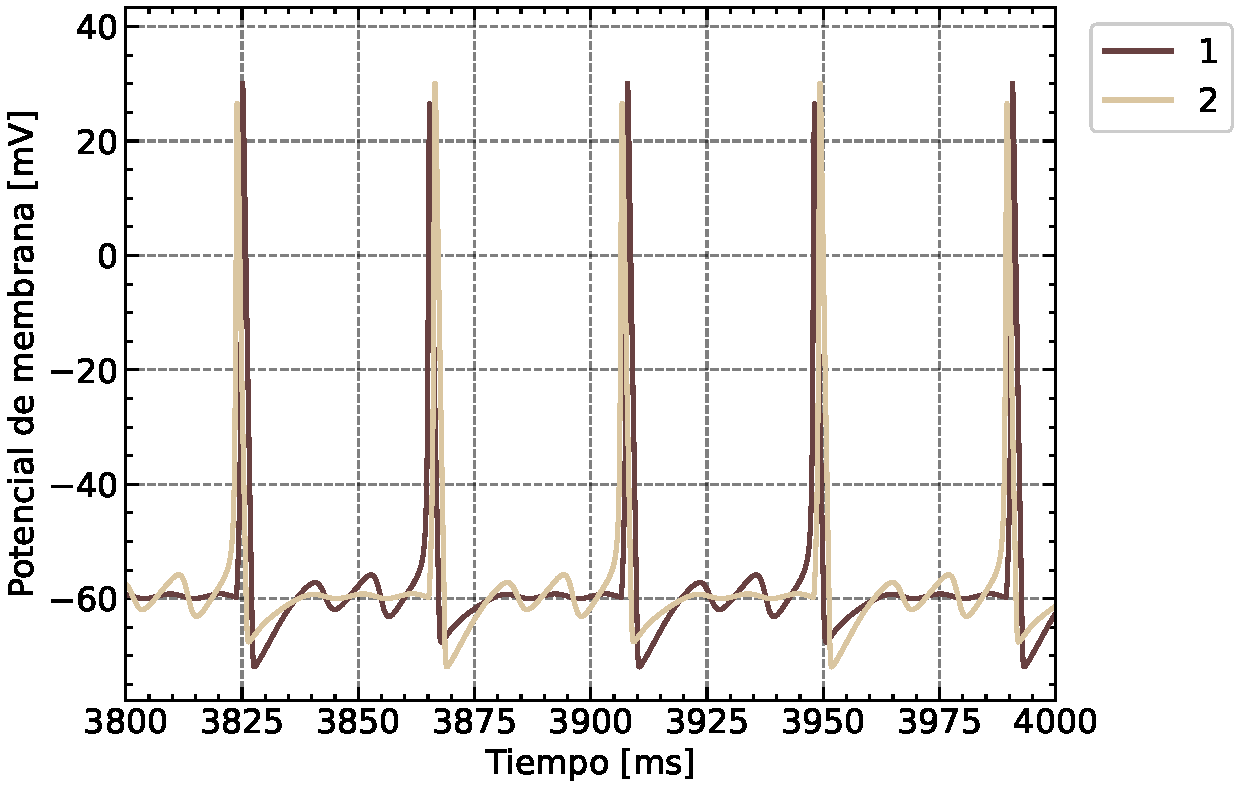
\includegraphics[width=0.45\textwidth]{figuras/excitatorio.pdf}
    \caption{dinámica de 2 neuronas de Hodgkin-Huxley con acoplamiento excitatorio para un valor de \(g_\text{syn} =\) \SI{0.45}{\milli\siemens\per \centi\meter\squared} y \(V_\text{syn} =\) \SI{0}{\milli\volt}.}
    \label{fig:ej1_exc_dinamica}    
\end{figure}

\begin{figure} [htbp]
    \centering
    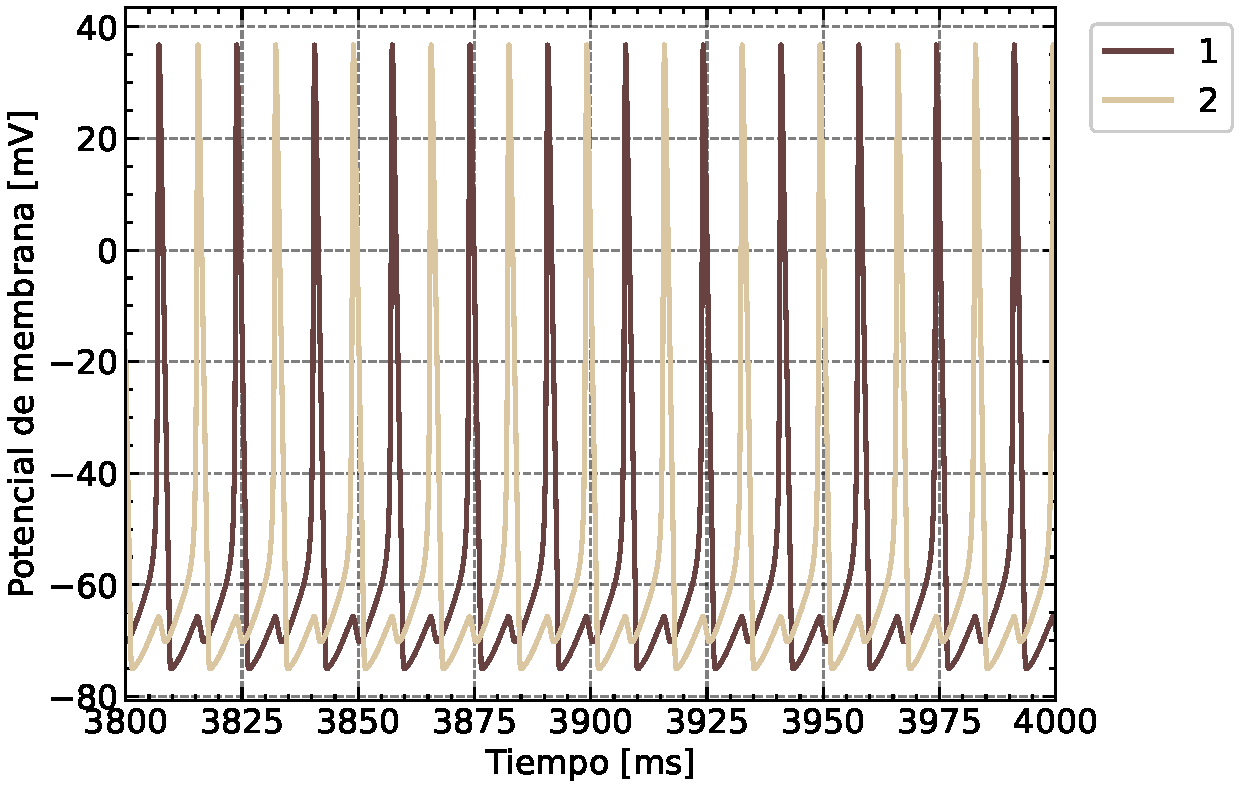
\includegraphics[width=0.45\textwidth]{figuras/inhibitorio.pdf}
    \caption{dinámica de 2 neuronas de Hodgkin-Huxley con acoplamiento inhibitorio para un valor de \(g_\text{syn} =\) \SI{0.45}{\milli\siemens\per \centi\meter\squared} y \(V_\text{syn} =\) \SI{-80}{\milli\volt}.}
    \label{fig:ej1_inh_dinamica}
\end{figure}

Para un valor de \(g_\text{syn} =\) \SI{0.45}{\milli\siemens\per \centi\meter\squared}, en el caso excitatorio con \(V_\text{syn} =\) \SI{0}{\milli\volt}(Figura \ref{fig:ej1_exc_dinamica}), se visualiza que las neuronas oscilan en fase, en cambio en el caso inhibitorio con \(V_\text{syn} =\) \SI{-80}{\milli\volt} (Figura \ref{fig:ej1_inh_dinamica}) se observa que las neuronas oscilan en contrafase. Para observar la dependencia tanto del desfasaje como la tasa de disparo del sistema en función de \(g_\text{syn}\) se realizó un barrido con 30 valores en el rango de \SI{0}{\milli\siemens\per \centi\meter\squared}, que se corresponde a 2 neuronas independientes sin interacción, a \SI{2}{\milli\siemens\per \centi\meter\squared}, dejando evolucionar el sistema hasta \SI{4}{\second}, en donde se supone que el sistema alcanzó un régimen estacionario. Los resultados se muestran en la Figura \ref{fig:ej1_barrido}.

\begin{figure} [htbp]
    \centering
    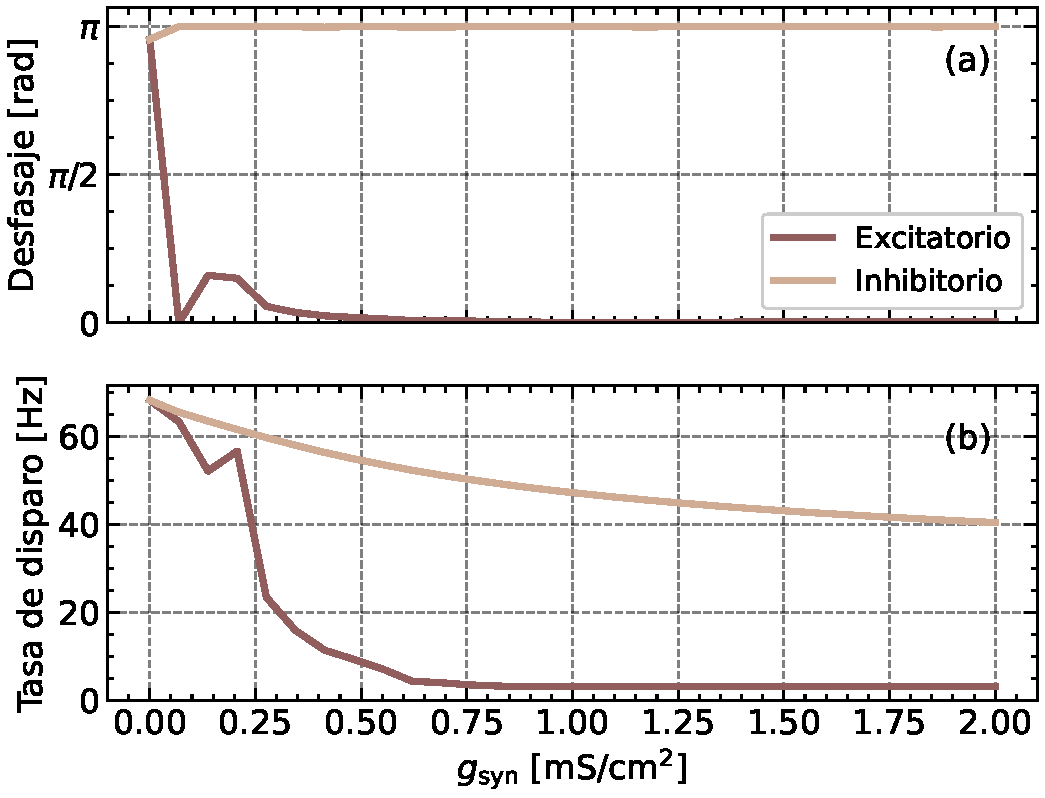
\includegraphics[width=0.45\textwidth]{figuras/barrido_nsyn.pdf}
    \caption{desfasaje y tasa de disparo en función de \(g_\text{syn}\) para el caso excitatorio y inhibitorio.}
    \label{fig:ej1_barrido}
\end{figure}

Se observa que para el caso excitatorio (Figura \ref{fig:ej1_barrido}a) el desfasaje es 0 para todos los valores de \(g_\text{syn}\), excepto en un entorno cercano a \(g_\text{syn} \sim 0.25\), sin embargo este último es cercano a 0 y podría deberse a un error numérico en la simulación. La tasa de disparo disminuye de manera abrupta para valores de \(g_\text{syn} \leq 0.5\), luego la tendencia cambia pero la tasa de disparo sigue disminuyendo. En el caso inhibitorio (Figura \ref{fig:ej1_barrido}b) se observa que el desfasaje es 180 para todos los valores de \(g_\text{syn}\) y la tasa de disparo disminuye de manera suave a medida que \(g_\text{syn}\) aumenta, tendiendo a un valor cercano a \SI{40}{\hertz} para los valores más altos de \(g_\text{syn}\) analizados.


\subsection*{Ejercicio 2}
Se considera un modelo de dos poblaciones de neuronas descritas por un modelo de tasa de disparo con una relación f-I semilineal de la forma 

\begin{eqnarray*}
    \tau \partial_t h_e  &=& -h_e + g_{ee} f_e - g_{ei} f_i + I_e, \\
    \tau \partial_t h_i  &=& -h_i + g_{ie} f_e - g_{ii} f_i + I_i,
\end{eqnarray*}

\noindent donde \(f_a = S(h_a)\) (\(a = e, i\)) con \(S(x) = x \Theta(x)\), siendo \(\Theta\) la función de Heaviside. 

Notar que si \(h_i < 0\) y \(h_e < 0\) entonces el sistema se desacopla por lo que no hay cambio de actividad. Luego si \(h_i < 0\) pero \(h_e > 0\), o viceversa, el sistema evoluciona incrementando la actividad de la variable negativa hasta llegar a un valor positivo. Por lo tanto para que el sistema pueda ser estable se analizan los casos en que \(h_i > 0\) y \(h_e > 0\). De este modo, el sistema resultado

\begin{eqnarray*}
    \tau \partial_t h_e  &=& -h_e + g_{ee} h_e - g_{ei} h_i + I_e, \\
    \tau \partial_t h_i  &=& -h_i + g_{ie} h_e - g_{ii} h_i + I_i,
\end{eqnarray*}

\noindent y como se quieren buscar soluciones estacionarias se tiene que \(\partial_t h_e = \partial_t h_i = 0\), por lo que se obtienen que las neuclinas del sistema son

\begin{eqnarray*}
    0  &=& f(h_e, h_i) = -h_e + g_{ee} h_e - g_{ei} h_i + I_e\\
    0  &=& g(h_e, h_i) = -h_i + g_{ie} h_e - g_{ii} h_i + I_i.
\end{eqnarray*}

Notar que las neuclinas son rectas en el espacio \((h_e, h_i)\) y se intersectan si las pendientes no son iguales. Se analiza el caso en que las pendientes no son iguales y se analiza como cambian las neuclinas frente a una perturbación en torno a un punto de estabilidad. 

Si se linealiza la perturbación \(\overline{\epsilon} = (\delta h_e, \delta h_i)\) en torno a un punto de estabilidad \((h_e^*, h_i^*)\) y se escribe de manera matricial, se obtiene que 

\begin{equation*}
    \frac{\partial \overline{\epsilon}}{\partial t} = \mathbf{A} \overline{\epsilon},
\end{equation*}

\noindent donde 

\begin{equation*}
    \mathbf{A} = \begin{pmatrix}
        \partial_{h_e} f(h_e, h_i) & \partial_{h_i} f(h_e, h_i) \\
        \partial_{h_e} g(h_e, h_i) & \partial_{h_i}g(h_e, h_i)
    \end{pmatrix}.
\end{equation*}

Por lo tanto, se convierte en un problema de autovalores, en donde para que sea estable se requiere que la parte real de los autovalores sea negativa. Se puede ver que los autovalores estan dados por \( \lambda = \frac{1}{2} (T \pm \sqrt{T^2-4D})\), donde \(T = Tr(A)\) y \(D = \text{det}(A)\), y se tiene que el sistema es estable si \(T < 0\) y \(D > 0\).

Particularizando para el sistema dado, se tiene que

\begin{equation}
    \mathbf{A} = \begin{pmatrix}
        g_{ee} - 1 & -g_{ei} \\
        g_{ie} & -g_{ii} - 1
    \end{pmatrix},
\end{equation}

además, se tiene que \( T = g_{ee} - g_{ii} -2\) y \(D = 1 -g_{ee} - g_{ee}g_{ii} + g_{ii} + g_{ie}g_{ei}\). Imponiendo la condición \(T < 0\) se tiene que

\begin{equation*}
    g_{ee} - g_{ii} < 2,
\end{equation*}
\noindent y para que sea estable se requiere que \(D > 0\), por lo que se tiene que

\begin{eqnarray*}
    1 - g_{ee} - g_{ee}g_{ii} + g_{ii} + g_{ie}g_{ei} &>& 0, \\
    g_{ee} - g_{ii} < 1 - g_{ee}g_{ii} + g_{ie}g_{ei} &<& 2\\,
\end{eqnarray*}

\noindent de esta ultima se obtiene \(g_{ie} g_{ei} - g_{ee}g_{ii} < 1\). 

\end{document}
